\documentclass[ % ドキュメントクラス
  uplatex,%upLaTeXを使う
  a5paper,%A5サイズにする
  papersize%紙のサイズがデフォルトと違う場合、PDFにうまく伝える
]{jsbook}

%% フォント関連
\usepackage[T1]{fontenc} % フォントでT1を使うこと
\usepackage{textcomp} % フォントでTS1を使うこと
\usepackage[utf8x]{inputenc} % ファイルがUTF8であること
\usepackage{newpxtext,newpxmath} % ローマンと数式の字体をPalatinoに基づいた新PXフォントで
\usepackage{zi4}%等幅フォントをInconsolataで
\usepackage[multi,deluxe,jis2004]{otf}
\usepackage[prefernoncjk]{pxcjkcat} % なるべく「半角」扱いで。


%% 図表など
% 図の読みこみのために
\usepackage[dvipdfmx, hiresbb]{graphicx, xcolor}
\usepackage{booktabs} % 表の横罫線
\usepackage{lscape}  % 表などを90度回転させる

%% 囲み枠
\usepackage{tcolorbox}
\tcbuselibrary{breakable} % ページをまたいで分割できるように
\tcbuselibrary{skins} % さまざまな skin を準備
\tcbuselibrary{theorems} % 定理環境

% 枠の定義
\newtcolorbox{summary}{
  sharp corners, % 角を丸くしない
  boxrule=0pt, % ボックスの罫線なし
  colback=green!20!white, % ボックスの背景色
}

\newtcolorbox{note}[1]{
  breakable, % ページをまたいでボックスを分割
  before skip=20pt plus 2pt minus 2pt, % ボックスの前の空き
  after skip=20pt plus 2pt minus 2pt, % ボックスの後の空き
  boxrule=0.4pt, % ボックスの罫線の太さ
  colframe=black!95, % フレームの色
  colback=white!95, % ボックスの背景色
  fonttitle=\gtfamily\bfseries, % タイトルのフォント
  title=#1 % タイトルのテキスト
}

% 参考情報を出力する命令を作る
\newtcbox{mysbox}{ % box を作る命令
  boxrule=0.4pt, % ボックスの罫線の太さ
  colframe=black, % フレームの色
  colback=black!10, % ボックスの背景色
  top=0mm, 
  bottom=0mm, 
  left=0mm, 
  right=0mm, 
  on line, arc=0.5mm}
\newcommand{\sanko}[1]{%
  \begin{itemize}
    \item[\mysbox{\small\gtfamily 参考}] #1
  \end{itemize}
}

% エピグラフ
\usepackage{epigraph}
\setlength{\epigraphwidth}{.6\textwidth}


%% ソースコードの出力
\usepackage{listings}
\lstset{ % 色々な設定
    language=R, % プログラミング言語名(ここではR言語)
    basicstyle=\ttfamily, % 基本的にタイプライター体にする
    numbers=left, % 左側に行番号を表示
    numberstyle=\small, % 行番号は小さめに
    numbersep=16pt, % 行番号をどれだけ離すか
    % showspaces=true,% スペースを表示したければtrueにする 
    xleftmargin=25pt, % 左側のマージン
    frame=single, %ソースコードを囲むフレーム
    framesep=10pt, %フレームとコードの間隔
    backgroundcolor=\color[gray]{0.95}, % 背景色
    breaklines=true % 長い行は改行する
}
\renewcommand{\lstlistingname}{ソースコード}


%% misc
\usepackage{okumacro} % 圏点などのために
\usepackage{pxrubrica} % ルビをつける(okumacroのrubyは使わない)


%% hyperrefの設定
\usepackage[dvipdfmx, %
   bookmarks=true, %PDFにしおりをつける
   bookmarksnumbered=true, %しおりに節番号などをつける
   colorlinks=false, %リンクには色をつけない
   hyperfootnotes=false, %脚注からのリンクを作らない
   pdfborder={0 0 0}, % リンクの枠なし
   pdfpagelayout=TwoPageRight, %奇数頁が右側になるような見開きモードで開く
   pdfpagemode=UseNone]{hyperref}

% PDFにしたときのしおりの文字化けを防ぐ
\usepackage{pxjahyper}

%% 索引
\usepackage{makeidx}
\makeindex


\begin{document}

% 標題
\begin{titlepage}
  \vspace*{10mm}
  \noindent{\fontsize{30pt}{48pt}\gtfamily\bfseries タイトル}
  \vfill

  \begin{flushright}
    {\gtfamily\bfseries\huge 著者 名}
  \end{flushright}

  \vspace{20mm}
\end{titlepage}
% 標題終わり

\frontmatter

\chapter{序}

ここには序の内容が入る。

\tableofcontents % 目次

\mainmatter

\chapter{最初の章}

\epigraph{エピグラフの文章が入る。}{エピグラフの出典が入る。}

\begin{summary}
ここは最初の章の概要の文章が入る。
ここは最初の章の概要の文章が入る。
ここは最初の章の概要の文章が入る。
ここは最初の章の概要の文章が入る。
ここは最初の章の概要の文章が入る。
\end{summary}

\section{最初の節の見出し}

ここは最初の節の文章が入る。
ここは最初の節の文章が入る。
ここは最初の節の文章が入る。
ここは最初の節の文章が入る。
ここは最初の節の文章が入る。

\subsection{最初の小節の見出し}

ここには最初の小節の文章が入る。
ここには最初の小節の文章が入る。
ここには最初の小節の文章が入る。
ここには最初の小節の文章が入る。
ここには最初の小節の文章が入る。

\subsubsection{最初の小々節の見出し}

ここには文章が入る。
ここには文章が入る。
ここには文章が入る。
ここには文章が入る。
ここには文章が入る。

\subsubsection{とってもとってもとってもとってもとってもとってもとってもとってもとっても長い小々節の見出し}

ここには文章が入る。
ここには文章が入る。
ここには文章が入る。
ここには文章が入る。
ここには文章が入る。

\paragraph{段落の見出し}

ここには文章が入る。
ここには文章が入る。
ここには文章が入る。
ここには文章が入る。
ここには文章が入る。

\paragraph{とってもとってもとってもとっても長い段落の見出し}

ここには文章が入る。
ここには文章が入る。
ここには文章が入る。
ここには文章が入る。
ここには文章が入る。

\subsection{第二の小節の見出し}

ここには第二の小節の文章が入る。
ここには第二の小節の文章が入る。
ここには第二の小節の文章が入る。
ここには第二の小節の文章が入る。
ここには第二の小節の文章が入る。

\section{第二の節の見出し}

ここは第二の節の文章が入る。
ここは第二の節の文章が入る。
ここは第二の節の文章が入る。
ここは第二の節の文章が入る。
ここは第二の節の文章が入る。

\chapter{解説}

\begin{summary}
この章では、\LaTeX で文章を書くときによく使う命令などを紹介する。
あわせて、本テンプレートで定義してある命令などについても紹介する。
\end{summary}

\section{タイプセットのための準備}

\subsection{環境構築}

\LaTeX の環境を構築するには、\TeX Live をインストールするのが手軽である。
詳しいインストール方法は、\TeX wiki の 
\url{https://texwiki.texjp.org/?TeX%20Live} に書かれている。

また、奥村・黒木〔著〕『美文書入門第7版』(以下、『美文書入門』)に付属している DVD からインストールすることもできる。

\subsection{ソースファイルの作成}

\subsubsection{ソースファイルの文字コード}
\TeX のソースファイルの文字コードは、UTF-8 にする。
プリアンブルには、必ず \verb|\usepackage[utf8]{inputenc}| と書いておく。

\subsubsection{ソースファイル編集用のソフト}
自分は、ソースファイルの編集とタイプセットには、
(1) TeXworks か、(2) Atom を使っている。
いずれもテキストエディタとして用いることができ、ソフト上から簡単にタイプセットすることができる。

ただし、(2) のAtom はそのままではタイプセットができない。
このため、タイプセット用の拡張パッケージとして \texttt{latex} を導入しておく必要がある。

また、以下のパッケージを導入しておくと、編集の際に便利である。

\begin{itemize}
  \item \texttt{language-latex}: 構文ハイライトを行う。
  \item \texttt{latexer}: 命令などの自動補完を行う。
  \item \texttt{pdf-view}: Atom 上で PDF を表示するためのもので、できあがった PDF を確認するときに使える。
\end{itemize}

なお、Atom の使用については、
\TeX wiki の \url{https://texwiki.texjp.org/?Atom} に詳しい情報がある。


\subsection{タイプセットの流れ}
タイプセットの際には、まず up\LaTeX でソースファイルから DVI ファイルを作るようにしている。
そして、dvipdfmx を使って、DVI ファイルから PDF にしている。

ただ、実際にタイプセットするときは、
up\LaTeX と dvipdfmx を個別に実行する必要はない。
ptex2pdf というものが用意されているので、
こちらを使うようにしている。
ptex2pdf を使うと、
up\LaTeX と dvipdfmx が順次実行され、
ソースファイルから PDF が作成される。
TeXworks を使うにせよ、Atom を使うにせよ、
ptex2pdf を呼び出すようにしておけば、
一発でタイプセットできる。


\section{フォント関連}

\subsection{エンコーディング}
プリアンブルにおいて、
\verb|\usepackage[T1]{fontenc}| と \verb|\usepackage{textcomp}| を
指定しておく。
こうすることによって、ソースコード上に入力された
アクセント付きの文字などをそのまま出すことが
できる\footnote{“é” と出力したい場合、\verb|``\'{e}''| とわざわざ入力する必要はなく、直接 \verb|“é” |と入力すればよい。}。

また、プリアンブルにおいて、
\verb|\usepackage[prefernoncjk]{pxcjkcat}|と指定しておけば、
全角でも半角でも出力できる文字が、
なるべく半角あつかいで出力されるようになる。
これを指定しないと、
“coup d’état”が
“\withcjktokenforced{coup d’état}”
のように出力されてしまう。

このあたりのことの詳細は、
『美文書入門』第7版の12.4節に載っている。

\subsection{欧文フォント}
Palatino に基づいた新PXフォントを使うために、
\texttt{newpxtext}, \texttt{newpxmath} パッケージを
読みこんでいる。

また、等幅フォントを Inconsolata にするために、\texttt{zi4} パッケージを読みこんでいる。


\subsection{日本語フォント}

\texttt{otf} パッケージを読みこむことで、
日本語フォントを色々使えるようにしている。

この \texttt{otf} パッケージに \texttt{deluxe} オプションをつけると、以下のように色々な書体が使えるようになる。

\begin{itemize}
  \item \verb|{\mcfamily\bfseries 太明朝体}| → {\mcfamily\bfseries 太明朝体}
  \item \verb|{\gtfamily ゴシック体}| → {\gtfamily ゴシック体}
  \item \verb|{\gtfamily\bfseries 太ゴシック体}| → {\gtfamily\bfseries 太ゴシック体}
  \item \verb|{\gtfamily\ebseries 極太ゴシック体}| → {\gtfamily\ebseries 極太ゴシック体} 
  \item \verb|{\mgfamily 丸ゴシック体}| → {\mgfamily 丸ゴシック体} 
\end{itemize}


\section{図表}

\subsection{図の出力}
図を読みこんで出力するために、
プリアンブルで \verb|\usepackage[dvipdfmx, hiresbb]{graphicx, xcolor}| を指定している。

図は基本的に PDF で用意しておくのが便利である。

\verb|barplot01.pdf| という図を出力したい場合は、
\verb|figure| 環境の中に \verb|\includegraphics{hoge.pdf}| 
という命令を入れる。
\verb|\includegraphics| の後に、
\verb|\caption| という命令を入れることで、
キャプションを表示することができる。

また、\verb|\label{fg:barplot-example}| という
ラベルを \verb|figure| 環境の中に置いておけば、
\verb|図\ref{fg:barplot-example}| で
図の番号「図\ref{fg:barplot-example}」を
取得できる。

\begin{figure}[h]
  \centering
  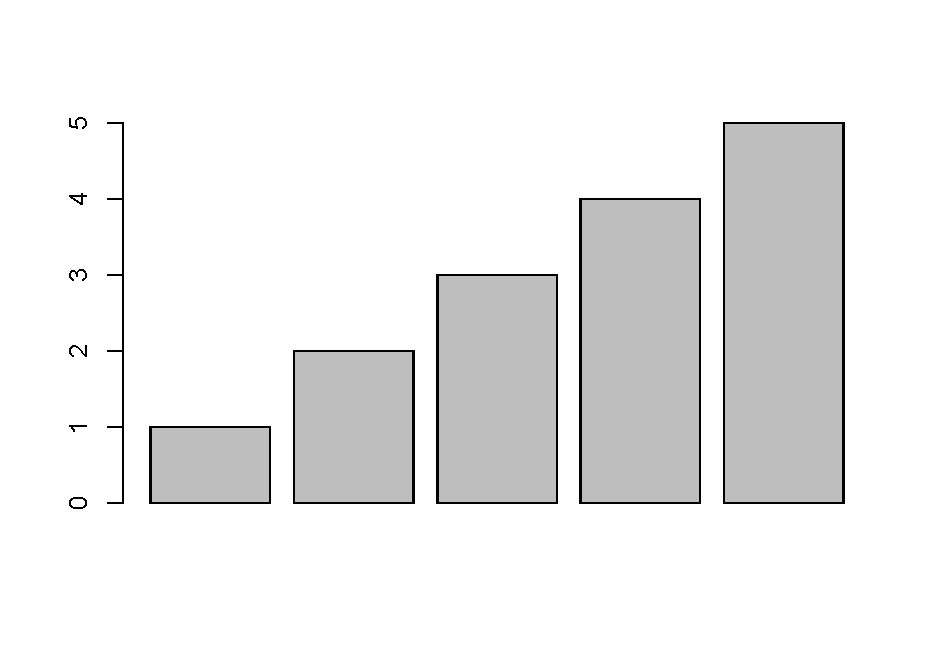
\includegraphics[width=0.8\hsize]{barplot01.pdf}
  \caption{これは図の例で、棒グラフが書かれている。}
  \label{fg:barplot-example}
\end{figure}


\subsection{表の出力}
表を出力するときには、\verb|table| 環境を使う。\verb|table| 環境の中に、\verb|tabular| 環境を記述することで表を作成する。
なお、横罫線を引くために、\texttt{booktabs} パッケージを使う。
縦罫線はなるべく引かない。


\verb|table| 環境の前に、
\verb|\caption| という命令を入れて、
キャプションを表示することができる。
なお、図の場合はキャプションを図の下に置くが、
表の場合はキャプションを表の上に置くのが普通である。

また、\verb|\label{tb:table-example}| という
ラベルを \verb|table| 環境の中に置いておけば、
\verb|表\ref{tb:table-example}| で
表の番号「表\ref{tb:table-example}」を
取得できる。

\begin{table}[h]
  \caption{これは表の例で、3行3列から成り立っている。}
  \label{tb:table-example}
  \begin{center}
    \begin{tabular}{lll} \toprule
      見出し1 & 見出し2 & 見出し3 \\ \midrule
      あああ & いいい & ううう \\
      かかか & ききき & くくく \\ \bottomrule
    \end{tabular}
  \end{center}
\end{table}

\subsection{横長の大きな図表}

横長の大きな図表を載せるときに、
90度回転させて表示させたいことがある。
この場合は、\texttt{lscape} パッケージが提供する
\verb|landscape| 環境を使う。
表\ref{tb:wide-table-example}がその例である。

\begin{landscape}
  \begin{table}
    \caption{かなり横長の表の例。}
    \label{tb:wide-table-example}
    \begin{center}
      \begin{tabular}{lllllllllllll} \toprule
        言語名   & 月曜日     & 火曜日      & 水曜日       & 木曜日        & 金曜日       & 土曜日      & 日曜日      \\ \midrule
        ドイツ語  & Montag  & Dienstag & Mittwoch  & Donnerstag & Freitag   & Samstag  & Sonntag  \\
        フランス語 & lundi   & mardi    & mercredi  & jeudi      & vendredi  & samedi   & dimanche \\
        英語    & Monday  & Tuesday  & Wednesday & Thursday   & Friday    & Saturday & Sunday   \\
        スペイン語 & lunes   & martes   & miércoles & jueves     & viernes   & sábado   & domingo  \\ \bottomrule
      \end{tabular}
    \end{center}
  \end{table}
\end{landscape}

\section{囲み枠}

囲み枠を作るには、\texttt{tcolorbox} パッケージを使うのが便利である。

このテンプレートでは、\verb|note| という環境を用意して、
コラム的な囲み記事を書くときに使えるようにしている。

\begin{note}{囲み記事のタイトル}
囲み記事の文章がここに入る。
囲み記事の文章がここに入る。
囲み記事の文章がここに入る。
囲み記事の文章がここに入る。
囲み記事の文章がここに入る。
囲み記事の文章がここに入る。
囲み記事の文章がここに入る。
囲み記事の文章がここに入る。
\end{note}

また、このテンプレートでは、以下のような参考情報を出力する命令として、\verb|\sanko| を用意してある。

\sanko{短い参考情報を提示するときのために使う。}


\section{ソースコードの出力}

シンタックスハイライトがなされたソースコードを出力するには、
\texttt{listings} パッケージを用いる。

\begin{lstlisting}[caption=簡単なプログラムの例, label=ls:example]
x <- c(24, 23, 15, 52, 63)
mean(x) # 平均を計算
\end{lstlisting}


\section{その他の文字装飾}

\subsection{圏点}
\kenten{圏点}を使うことで、語句を強調することができる。
\kenten{圏点}を出力するには、
\texttt{okumacro} パッケージを読みこんだ上で、
\verb|\kenten{圏点}| とする。 


\subsection{ルビ}
ルビをふるには、\texttt{pxrubrica} パッケージの \verb|\jruby| という命令を使う
\footnote{\texttt{pxrubrica} パッケージでは、 \verb|\ruby| という命令でルビをふる機能も付いているが、\texttt{okumacro} パッケージの \verb|\ruby| とかぶるため、用いないものとする。}。

基本的には、\verb#\jruby{漢字}{かん|じ}# の形で書く。
グループルビにしたければ、\verb|\jruby[g]{弥生}{やよい}| のように、\verb|[g]| をつける。

\begin{tcolorbox}[title=ルビの例, sidebyside, sidebyside align=top, righthand ratio=0.7]
\jruby{黄}{き}と\jruby{赤}{あか}と
\jruby{緑}{みどり}の
\jruby{高価}{こう|か}で
\jruby{貴重}{き|ちょう}なものを
\jruby{購入}{こう|にゅう}しました。
\jruby[g]{閑話休題}{それはさておき}、
\jruby[g]{昨日}{きのう}は
\jruby[g]{心太}{ところてん}を
ありがとう。
\tcblower
\begin{verbatim}
\jruby{黄}{き}と\jruby{赤}{あか}と
\jruby{緑}{みどり}の
\jruby{高価}{こう|か}で
\jruby{貴重}{き|ちょう}なものを
\jruby{購入}{こう|にゅう}しました。
\jruby[g]{閑話休題}{それはさておき}、
\jruby[g]{昨日}{きのう}は
\jruby[g]{心太}{ところてん}を
ありがとう。
\end{verbatim}
\end{tcolorbox}



\section{\texttt{hyperref}}
\texttt{hyperref} パッケージにより、PDF にリンクを貼ったり、
PDF にしおりをつけたりすることができる。

なお、日本語のしおりの文字化けを防ぐには、
プリアンブルで \verb|\usepackage{pxjahyper}| と記述する。

\section{索引}
索引をつけるには、プリアンブルで \verb|\usepackage{makeidx}| と
\verb|\makeindex| を宣言しておく。

\section{目次}

目次を出力したい場所に、\verb|\tableofcontents| と記述することで、目次を出力することができる。

\end{document}